\documentclass[dvipsnames]{beamer}
\usepackage[utf8]{inputenc}
\usepackage{listings}
\usepackage{comment}
\usepackage{soul}
%\usepackage{ulem}
\usepackage{subfig}
\setul{}{1pt}
\usepackage[oldenum, olditem]{paralist}
%allow even smaller text
\newcommand\tinytiny{\fontsize{4pt}{3}\selectfont}

\makeatletter
\let\old@lstKV@SwitchCases\lstKV@SwitchCases
\def\lstKV@SwitchCases#1#2#3{}
\makeatother
\usepackage{lstlinebgrd}
\makeatletter
\let\lstKV@SwitchCases\old@lstKV@SwitchCases

\lst@Key{numbers}{none}{%
    \def\lst@PlaceNumber{\lst@linebgrd}%
    \lstKV@SwitchCases{#1}%
    {none:\\%
     left:\def\lst@PlaceNumber{\llap{\normalfont
                \lst@numberstyle{\thelstnumber}\kern\lst@numbersep}\lst@linebgrd}\\%
     right:\def\lst@PlaceNumber{\rlap{\normalfont
                \kern\linewidth \kern\lst@numbersep
                \lst@numberstyle{\thelstnumber}}\lst@linebgrd}%
    }{\PackageError{Listings}{Numbers #1 unknown}\@ehc}}
\makeatother


\graphicspath{{logos/}}

\usepackage{tikz}
%disclaimer for Sandia. uncomment and the whole blob goes away @ b80c116300122
\def\sandid{SAND2020-7755 PE}

% \title{Performance Portability with Kokkos}
\title{The Kokkos Ecosystem}

%BAD misuse of author field
\author{C++ Performance Portability for the HPC Community}

%\author{
%  Jeff Miles \inst{1},
%  Christian Trott \inst{1}
%}
%\institute[shortinst]{\tiny \inst{1} Sandia National Laboratories, \inst{2} Oak Ridge National Laboratory \and \inst{3} Los Alamos National Laboratory}
%\institute[shortinst]{\tiny \inst{1} Sandia National Laboratories}

\usetheme{kokkos}

\newif\ifshort
\newif\ifmedium
\newif\iffull
\newif\ifnotoverview

\newcommand{\TutorialDirectory}{\texttt{Intro-Full}}
\newcommand{\ExerciseDirectory}[1]{\texttt{Exercises/#1/}}
\newcommand{\TutorialClone}{\texttt{Kokkos/kokkos-tutorials/\TutorialDirectory}}

\definecolor{darkgreen}{rgb}{0.0, 0.5, 0.0}
\definecolor{darkred}{rgb}{0.8, 0.0, 0.0}
\definecolor{orange}{rgb}{0.8, 0.33, 0.0}
\definecolor{purple}{rgb}{0.60, 0.20, 0.80}
\colorlet{bodyColor}{blue!20}
\colorlet{patternColor}{orange!30}
\colorlet{policyColor}{green!30}

% http://tex.stackexchange.com/questions/144448/color-a-text-line-in-a-code-lstlisting
\lstnewenvironment{code}[1][]%
{
  %with txfonts: OT1/txr/m/n/10
  %with default fonts: OT1/cmr/m/n/10
  %\fontfamily{cmr}\selectfont
  %\showthe\font
   \noindent
   \minipage{\linewidth}
   %\vspace{0.5\baselineskip}
   \lstset{mathescape, escapeinside={<@}{@>},
moredelim=**[is][{\btHL[fill=patternColor]}]{@pattern}{@pattern},
moredelim=**[is][{\btHL[fill=red!30]}]{@warning}{@warning},
moredelim=**[is][{\btHL[fill=policyColor]}]{@policy}{@policy},
moredelim=**[is][{\btHL[fill=bodyColor]}]{@body}{@body},
moredelim=**[is][{\btHL[fill=red!30]}]{@warning}{@warning},
moredelim=**[is][\color{black}]{@black}{@black},
moredelim=**[is][\color{blue}]{@blue}{@blue},
moredelim=**[is][\bf]{@bold}{@bold},
moredelim=**[is][\it]{@italic}{@italic},
moredelim=**[is][\color{boldblue}\bf]{@boldblue}{@boldblue},
moredelim=**[is][\color{red}]{@red}{@red},
moredelim=**[is][\color{green}]{@green}{@green},
moredelim=**[is][\color{gray}]{@gray}{@gray},
moredelim=**[is][\color{darkgreen}]{@darkgreen}{@darkgreen},
moredelim=**[is][\color{darkred}]{@darkred}{@darkred},
moredelim=**[is][\color{orange}]{@orange}{@orange},
moredelim=**[is][\color{purple}]{@purple}{@purple},
keywords={},
#1}
}
{
  \endminipage
  %\vspace{1.0\baselineskip}
}

\makeatletter
\newif\ifATOlinebackground
\lst@Key{linebackground}{\tiny}{\def\ATOlinebackground{#1}\global\ATOlinebackgroundtrue}
\makeatother

\lstnewenvironment{shell}[1][]{%
  \global\ATOlinebackgroundfalse
  \lstset{language=sh,%
    showstringspaces=false,
    aboveskip=0pt,
    frame=none,
    numbers=none,
    belowskip=2pt,
    breaklines=true,
    #1,
    }
  %\ifATOlinebackground
  \lstset{linebackgroundcolor={
    \ATOlinebackground
  }}
  %\fi
  }{}

\lstnewenvironment{cmake}[1][]{%
  \global\ATOlinebackgroundfalse
  \lstset{language=sh,%
    showstringspaces=false,
    aboveskip=0pt,
    frame=none,
    numbers=none,
    belowskip=2pt,
    breaklines=true,
    #1,
    }
  %\ifATOlinebackground
  \lstset{linebackgroundcolor={
    \ATOlinebackground
  }}
  %\fi
  }{}

\newcommand{\inlinecode}[1]{{\lstset{basicstyle=\ttfamily,keywordstyle={},showstringspaces=false}\lstinline$#1$}}
\newcommand{\inlineshell}[1]{{\lstset{basicstyle=\ttfamily,keywordstyle={},showstringspaces=false}\lstinline$#1$}}

\setbeamercolor{block title}{fg=white, bg=SandiaLightBlue}
\setbeamercolor{block body}{bg=lightgray}
\setbeamercolor{block title alerted}{fg=white, bg=SandiaRed}
\setbeamercolor{block body alerted}{bg=lightgray}



%\usepackage[texcoord,grid,gridunit=mm,gridcolor=red!10,subgridcolor=green!10]{eso-pic}
\usepackage[absolute,overlay]{textpos}





% http://tex.stackexchange.com/questions/8851/how-can-i-highlight-some-lines-from-source-code

\usepackage{pgf, pgffor}
\usepackage{listings}
\usepackage{lstlinebgrd} % see http://www.ctan.org/pkg/lstaddons

\makeatletter
%%%%%%%%%%%%%%%%%%%%%%%%%%%%%%%%%%%%%%%%%%%%%%%%%%%%%%%%%%%%%%%%%%%%%%%%%%%%%%
%
% \btIfInRange{number}{range list}{TRUE}{FALSE}
%
% Test in int number <number> is element of a (comma separated) list of ranges
% (such as: {1,3-5,7,10-12,14}) and processes <TRUE> or <FALSE> respectively

\newcount\bt@rangea
\newcount\bt@rangeb

\newcommand\btIfInRange[2]{%
    \global\let\bt@inrange\@secondoftwo%
    \edef\bt@rangelist{#2}%
    \foreach \range in \bt@rangelist {%
        \afterassignment\bt@getrangeb%
        \bt@rangea=0\range\relax%
        \pgfmathtruncatemacro\result{ ( #1 >= \bt@rangea) && (#1 <= \bt@rangeb) }%
        \ifnum\result=1\relax%
            \breakforeach%
            \global\let\bt@inrange\@firstoftwo%
        \fi%
    }%
    \bt@inrange%
}
\newcommand\bt@getrangeb{%
    \@ifnextchar\relax%
        {\bt@rangeb=\bt@rangea}%
        {\@getrangeb}%
}
\def\@getrangeb-#1\relax{%
    \ifx\relax#1\relax%
        \bt@rangeb=100000%   \maxdimen is too large for pgfmath
    \else%
        \bt@rangeb=#1\relax%
    \fi%
}

%%%%%%%%%%%%%%%%%%%%%%%%%%%%%%%%%%%%%%%%%%%%%%%%%%%%%%%%%%%%%%%%%%%%%%%%%%%%%%
%
% \btLstHL<overlay spec>{range list}
%
% TODO BUG: \btLstHL commands can not yet be accumulated if more than one overlay spec match.
%
\newcommand<>{\btLstHL}[2]{%
  \only#3{\btIfInRange{\value{lstnumber}}{#1}{\color{#2}\def\lst@linebgrdcmd{\color@block}}{\def\lst@linebgrdcmd####1####2####3{}}}%
}%
\makeatother






% http://tex.stackexchange.com/questions/15237/highlight-text-in-code-listing-while-also-keeping-syntax-highlighting
%\usepackage[T1]{fontenc}
%\usepackage{listings,xcolor,beramono}
\usepackage{tikz}

\makeatletter
\newenvironment{btHighlight}[1][]
{\begingroup\tikzset{bt@Highlight@par/.style={#1}}\begin{lrbox}{\@tempboxa}}
{\end{lrbox}\bt@HL@box[bt@Highlight@par]{\@tempboxa}\endgroup}

\newcommand\btHL[1][]{%
  \begin{btHighlight}[#1]\bgroup\aftergroup\bt@HL@endenv%
}
\def\bt@HL@endenv{%
  \end{btHighlight}%
  \egroup
}
\newcommand{\bt@HL@box}[2][]{%
  \tikz[#1]{%
    \pgfpathrectangle{\pgfpoint{1pt}{0pt}}{\pgfpoint{\wd #2}{\ht #2}}%
    \pgfusepath{use as bounding box}%
    \node[anchor=base west, fill=orange!30,outer sep=0pt,inner xsep=1pt, inner ysep=0pt, rounded corners=3pt, minimum height=\ht\strutbox+1pt,#1]{\raisebox{1pt}{\strut}\strut\usebox{#2}};
  }%
}
\makeatother



\usetikzlibrary{calc}
\usepackage{xparse}%  For \NewDocumentCommand

% tikzmark command, for shading over items
\newcommand{\tikzmark}[1]{\tikz[overlay,remember picture] \node (#1) {};}

\makeatletter
\NewDocumentCommand{\DrawBox}{s O{}}{%
    \tikz[overlay,remember picture]{
    \IfBooleanTF{#1}{%
        \coordinate (RightPoint) at ($(left |- right)+(\linewidth-\labelsep-\labelwidth,0.0)$);
    }{%
        \coordinate (RightPoint) at (right.east);
    }%
    \draw[red,#2]
      ($(left)+(-0.2em,0.9em)$) rectangle
      ($(RightPoint)+(0.2em,-0.3em)$);}
}

\NewDocumentCommand{\DrawBoxWide}{s O{}}{%
    \tikz[overlay,remember picture]{
    \IfBooleanTF{#1}{%
        \coordinate (RightPoint) at ($(left |- right)+(\linewidth-\labelsep-\labelwidth,0.0)$);
    }{%
        \coordinate (RightPoint) at (right.east);
    }%
    \draw[red,#2]
      ($(left)+(-\labelwidth,0.9em)$) rectangle
      ($(RightPoint)+(0.2em,-0.3em)$);}
}

\NewDocumentCommand{\DrawBoxWideBlack}{s O{}}{%
    \tikz[overlay,remember picture]{
    \IfBooleanTF{#1}{%
        \coordinate (RightPoint) at ($(left |- right)+(\linewidth-\labelsep-\labelwidth,0.0)$);
    }{%
        \coordinate (RightPoint) at (right.east);
    }%
    \draw[black,#2]
      ($(left)+(-\labelwidth,0.9em)$) rectangle
      ($(RightPoint)+(0.2em,-0.3em)$);}
}
\makeatother

\usetikzlibrary{positioning}

\usetikzlibrary{shapes}

\hypersetup{
    colorlinks=true,
    linkcolor=blue,
    filecolor=magenta,
    urlcolor=cyan,
}



\shorttrue
\mediumfalse
\fullfalse

\begin{document}


% \begin{frame}
%   \titlepage
% \end{frame}
% 
%==============================================================================

\begin{frame}{NVIDIA's NVLABS LOGISTICS (1)}

\textbf{\large SOFTWARE FOR LAB}

\vspace{10pt}

\textbf{Remote Desktop Software:} \\
\begin{itemize}
\item {Download NoMachine now for best performance from \\
 \textbf{\ul{www.nomachine.com/download}}}
\item {Alternatively you may use a VNC client or the provided browser-based VNC option}
\end{itemize}

\vspace{10pt}

\textbf{SSH Access Software (optional):}
\begin{itemize}
\item PuTTy for Windows can be downloaded from \textbf{\ul{www.putty.org}}
\item{Alternatively you may use a provided browser-based SSH option}
\end{itemize}

\end{frame}

%==============================================================================

\begin{frame}{NVIDIA's NVLABS LOGISTICS (2)}

\textbf{\Large CONNECTION INSTRUCTIONS}
\begin{itemize}
\item {Navigate to \textbf{\ul{nvlabs.qwiklab.com}}}
\item {Login or create a new account}
\item {Select the \textbf{Instructor-Led Hands-on Labs} Class}
\item {Find the lab called \textbf{Kokkos, ...}, select it, click Select, and finally click Start}
\item {After a short wait, lab instance Connection information will be shown}
\item {Please ask Lab Assistants for help!}
\end{itemize}

\end{frame}

%==============================================================================



\begin{frame}
	\titlepage
\end{frame}


% \begin{frame}{DOE ECP Acknowledgement}

% \textit{
% This research was supported by the Exascale Computing Project (17-SC-20-SC),
% a joint project of the U.S. Department of Energy’s Office of Science and National Nuclear Security Administration,
% responsible for delivering a capable exascale ecosystem, including software, applications, and hardware technology,
% to support the nation’s exascale computing imperative. 
% }

% \end{frame}

%==============================================================================
\ifnotoverview
\begin{frame}[fragile]

  \vspace{-10pt}

  {\Huge Introduction}

  \vspace{10pt}

  \textbf{Learning objectives:}
  \begin{itemize}
    \item{Why do we need Kokkos}
    \item{The Kokkos Ecosystem}
    \item{The Kokkos Team}
  \end{itemize}

  \vspace{-20pt}

\end{frame}
\fi

\begin{frame}[fragile]{The HPC Hardware Landscape}
  \begin{center}
    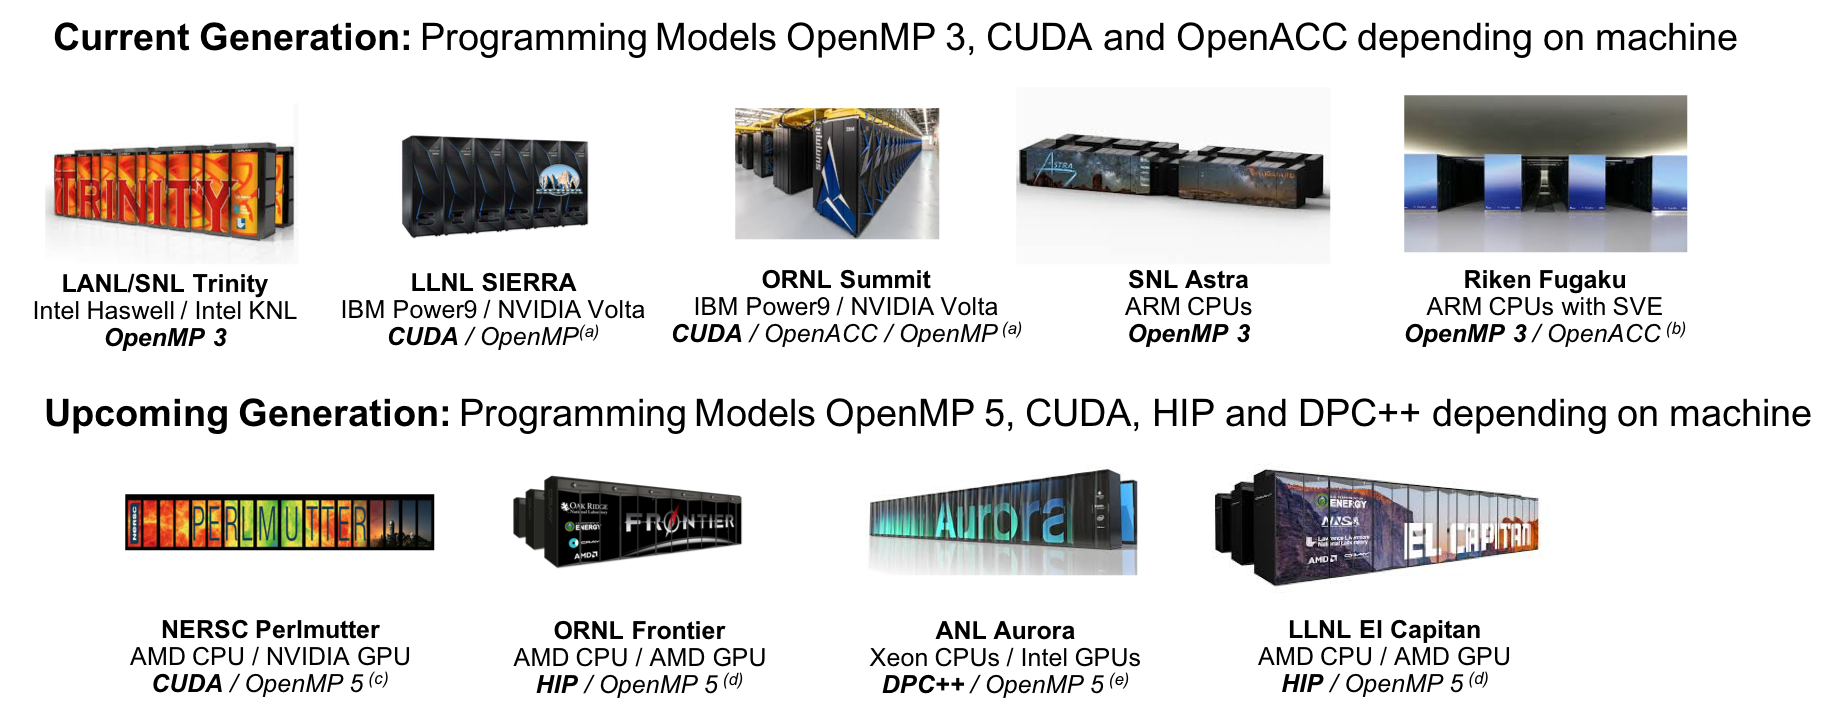
\includegraphics[width=1.05\textwidth]{figures/Architecture-Overview}
  \end{center}

  \begin{scriptsize}
  \emph{(a)} Initially not working. Now more robust for Fortran than C++, but getting better.

  \emph{(b)} Research effort.

  \emph{(c)} OpenMP 5 by NVIDIA.

  \emph{(d)} OpenMP 5 by HPE.

  \emph{(e)} OpenMP 5 by Intel.
  \end{scriptsize}

\end{frame}

\begin{frame}[fragile]{Cost of Coding}

\begin{block}{Industry Estimate}
A full time software engineer writes 10 lines of production code per hour: 20k LOC/year.
\end{block}

	\begin{itemize}
		\item Typical HPC production app: 300k-600k lines
			\begin{itemize}
				\item Sandia alone maintains a few dozen
			\end{itemize}
		\item Large Scientific Libraries:
			\begin{itemize}
				\item E3SM: 1,000k lines
				\item Trilinos: 4,000k lines
			\end{itemize}
	\end{itemize}

	\textbf{Conservative estimate:} need to rewrite 10\% of an app to switch Programming Model

	\pause

\begin{block}{Software Cost Switching Vendors}
Just switching Programming Models costs multiple person-years per app!
\end{block}

\end{frame}

\begin{frame}[fragile]{What is Kokkos?}
	\begin{itemize}
		\item A C++ Programming Model for Performance Portability
			\begin{itemize}
				\item Implemented as a template library on top CUDA, HIP, OpenMP, ...
				\item Aims to be descriptive not prescriptive
				\item Aligns with developments in the C++ standard
			\end{itemize}
		\item Expanding solution for common needs of modern science and engineering codes
			\begin{itemize}
				\item Math libraries based on Kokkos
				\item Tools for debugging, profiling and tuning
				\item Utilities for integration with Fortran and Python
			\end{itemize}
		\item It is an Open Source project with a growing community
			\begin{itemize}
				\item Maintained and developed at \url{https://github.com/kokkos}
				\item Hundreds of users at many large institutions
			\end{itemize}
	\end{itemize}
\end{frame}

\begin{frame}[fragile]{Kokkos at the Center}
  \begin{center}
    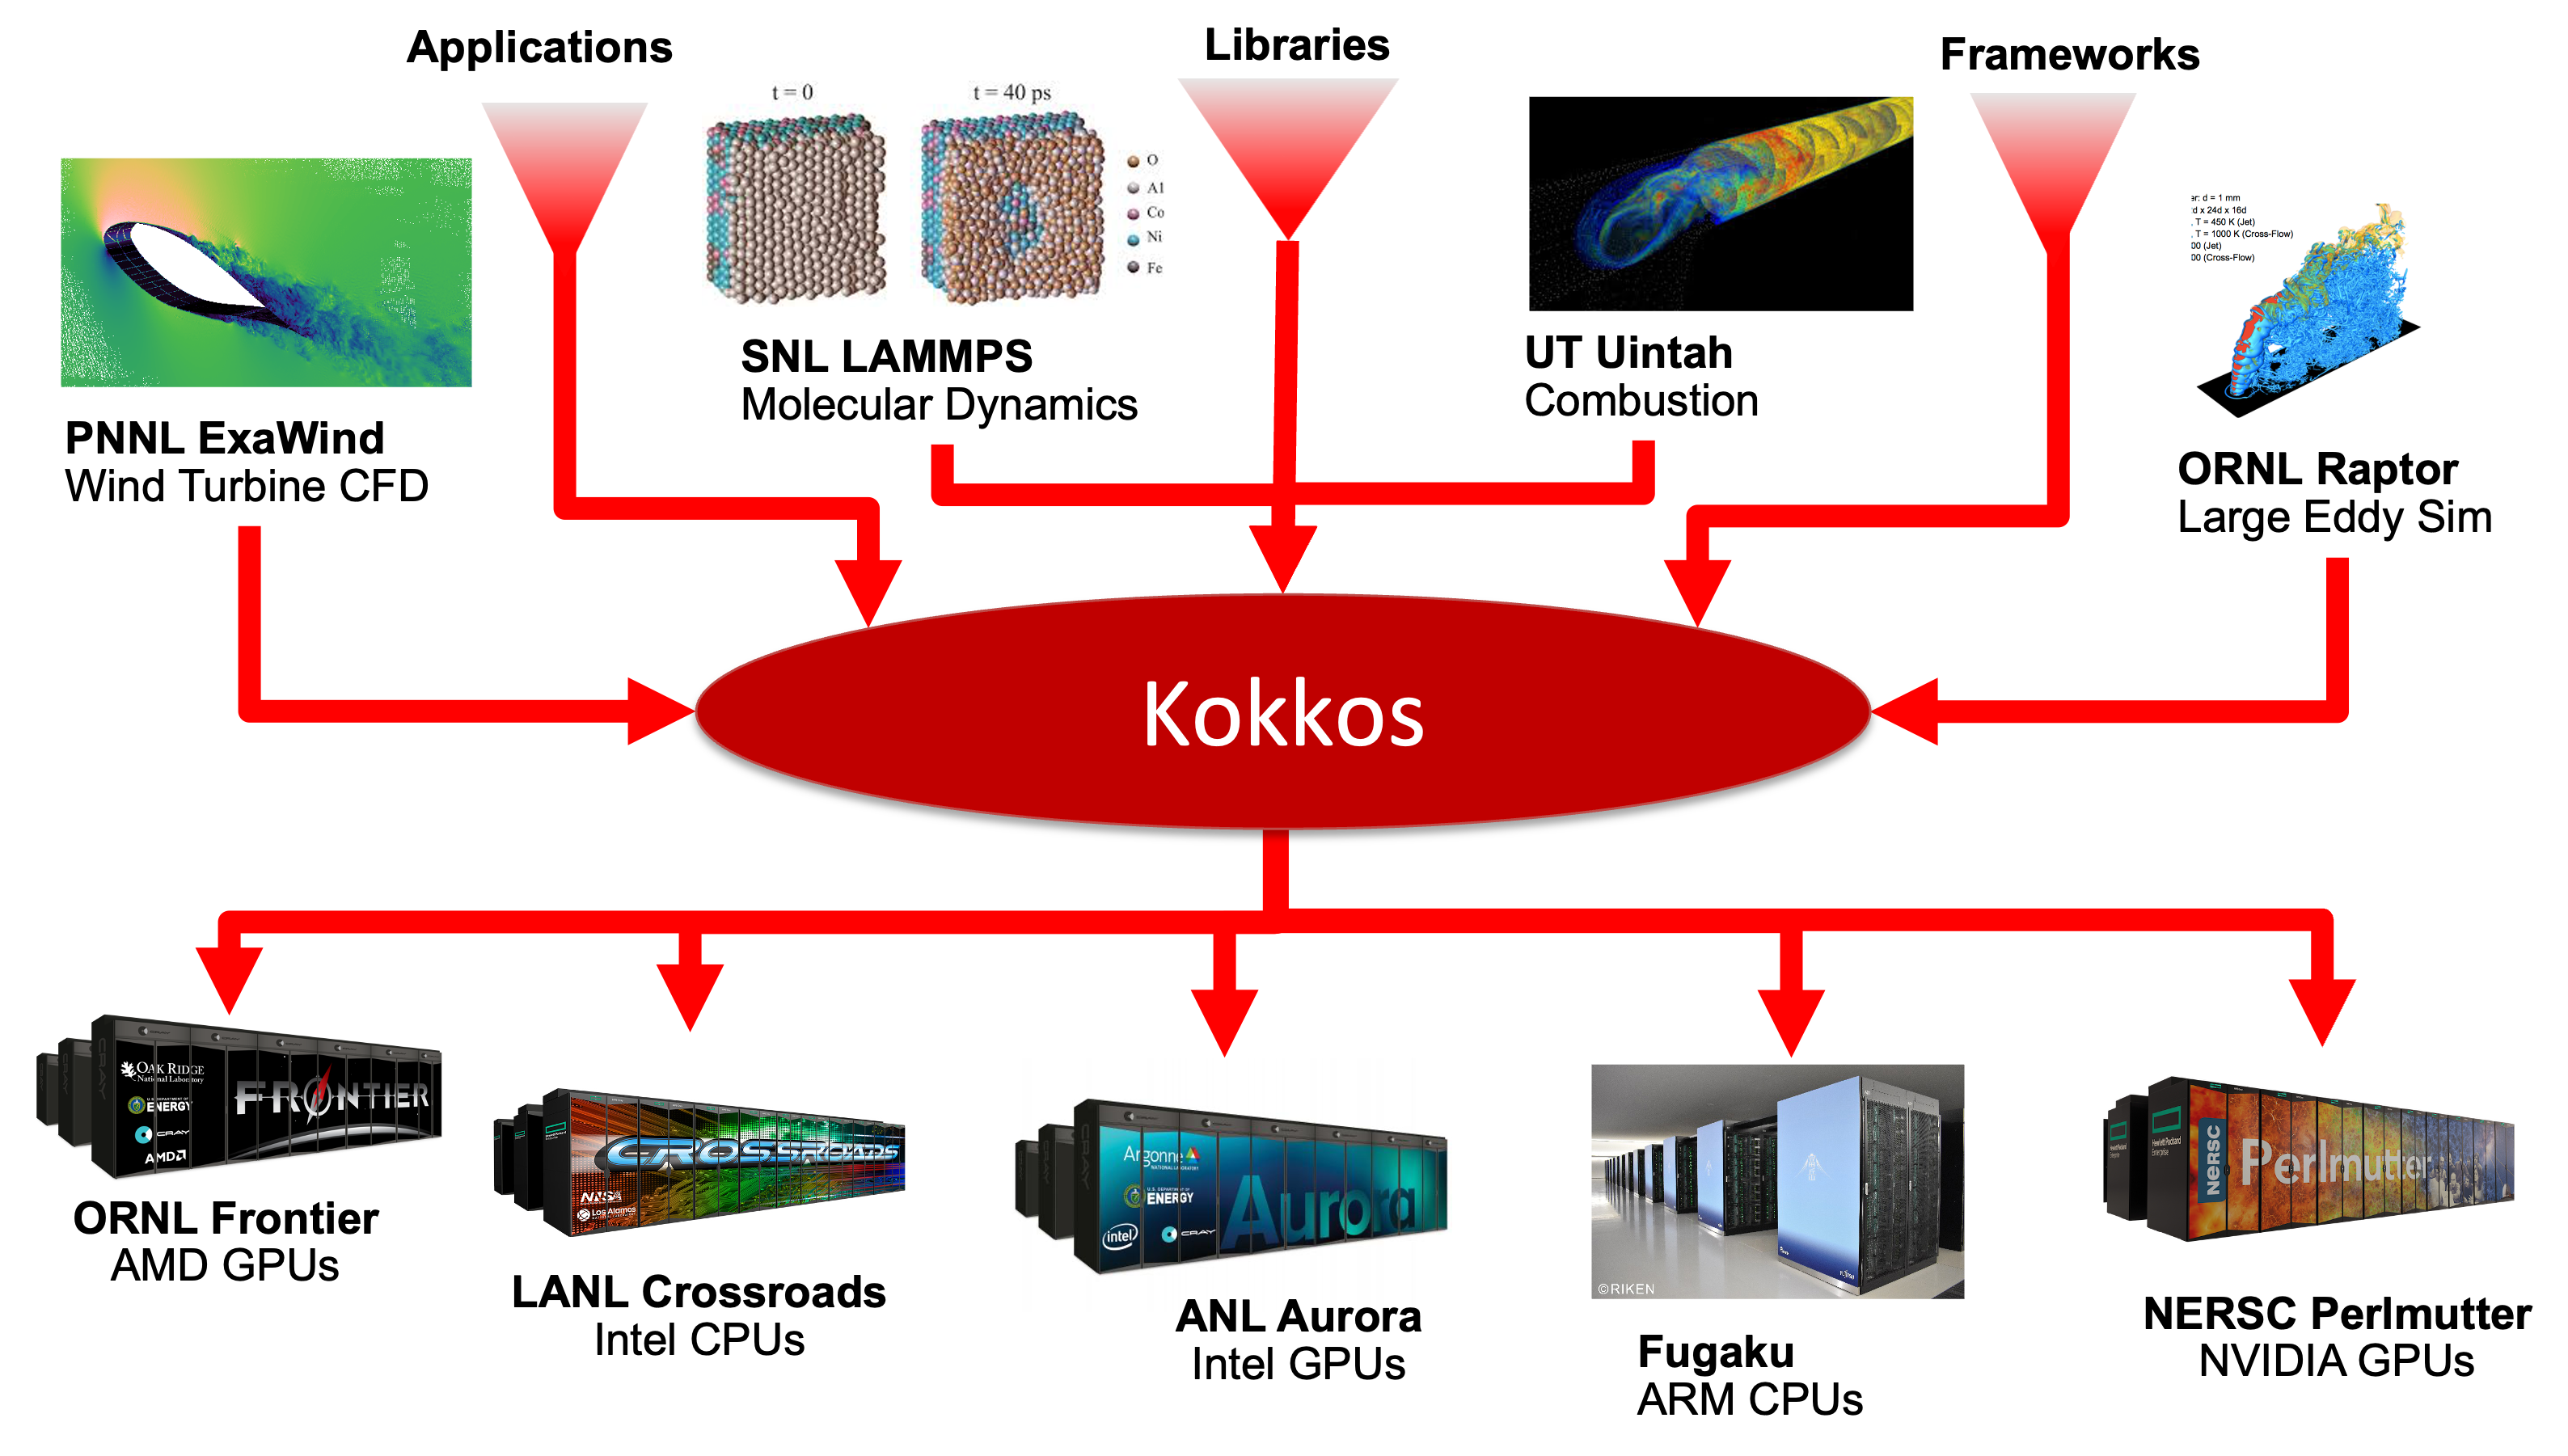
\includegraphics[width=1.05\textwidth]{figures/Kokkos-In-The-Middle-2024}
  \end{center}
\end{frame}

\begin{frame}[fragile]{The Kokkos Ecosystem}
  \begin{center}
    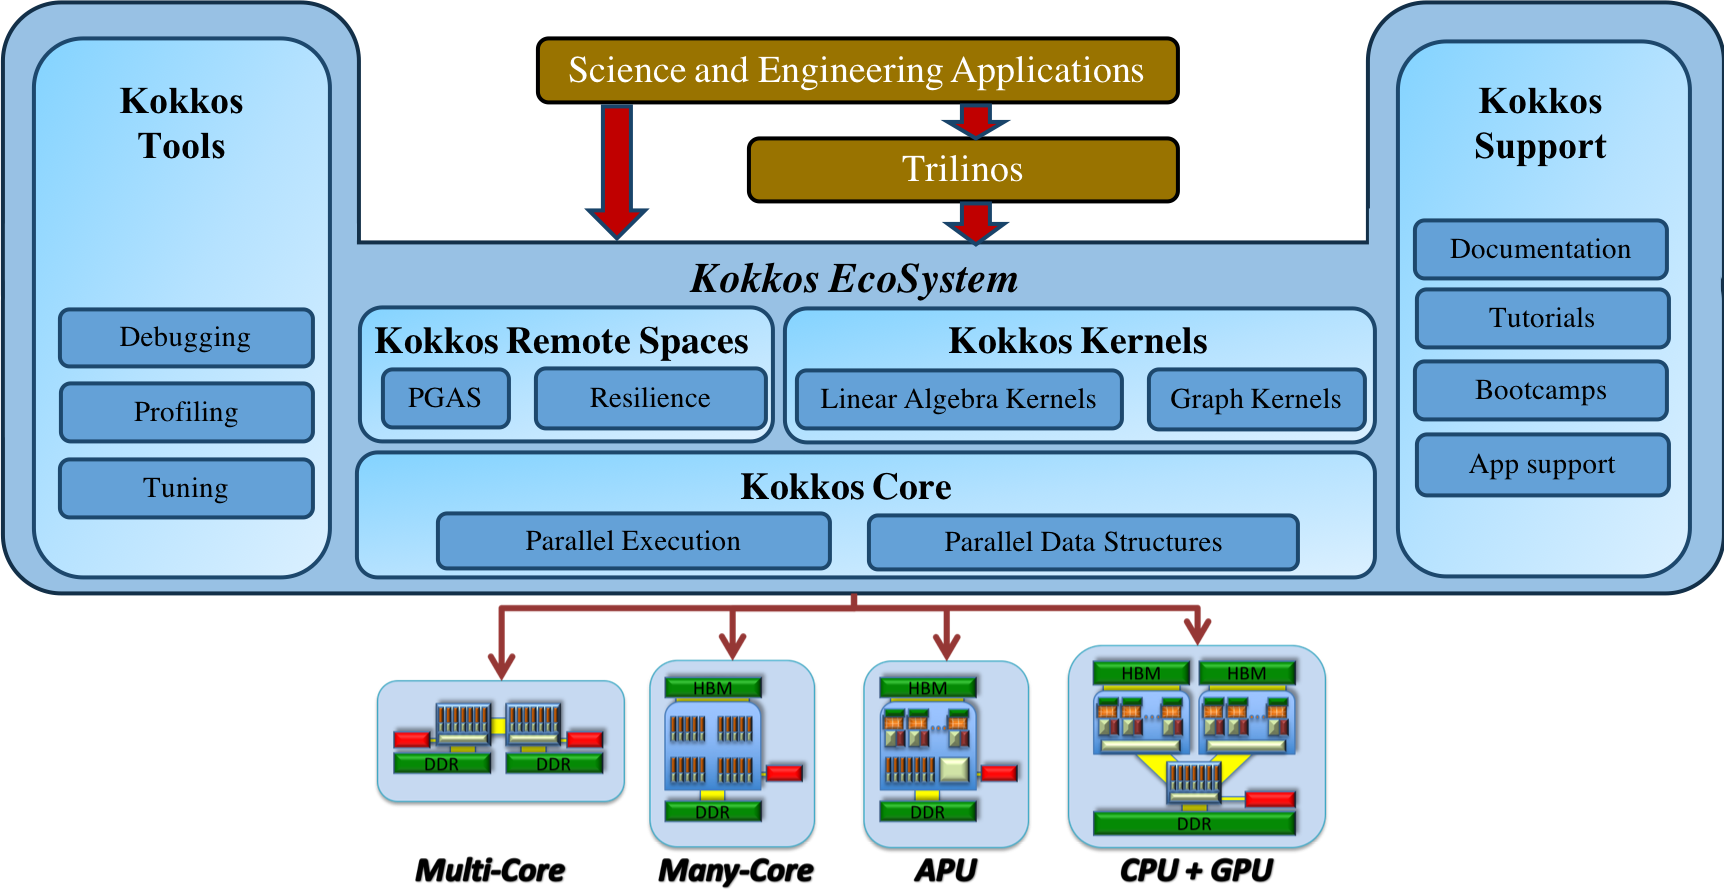
\includegraphics[width=1.05\textwidth]{figures/kokkos-eco-system}
  \end{center}
\end{frame}

\begin{frame}[fragile]{The Kokkos Team}
  \begin{center}
    
\includegraphics[width=0.9\textwidth]{figures/Kokkos-Team-2024}
  \end{center}
\end{frame}


\begin{frame}[fragile]{Kokkos and the C++ Standard}
  \textbf{Kokkos helps improve ISO C++}


	\vspace{-25pt}
\begin{center}                                                                                                                                    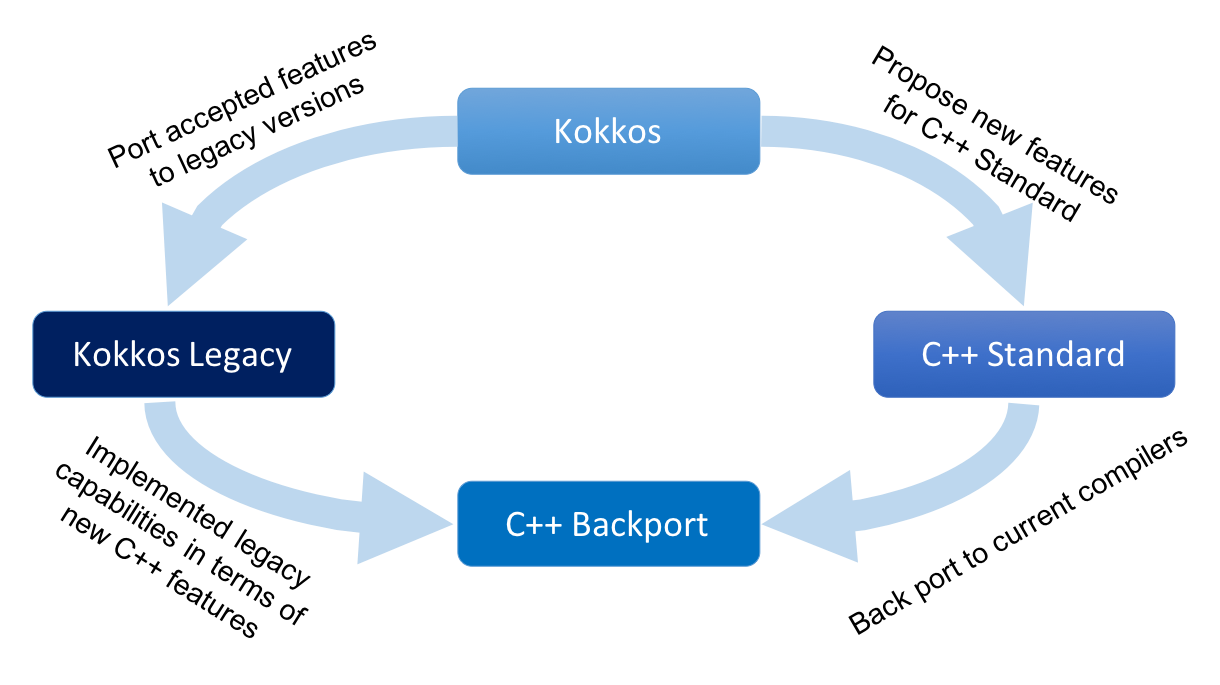
\includegraphics[width=1.05\textwidth]{figures/kokkos-cpp-standard}
\end{center}

	\vspace{-25pt}
\textit{Ten current or former Kokkos team members are members of the ISO C++ standard committee.}
\end{frame}

\iffull
\begin{frame}[fragile]{C++20 std::atomic\_ref}
	\textbf{C++11 std::atomic insufficient for HPC}
	\begin{itemize}
           \item Objects, not functions, with only atomic access
	   \item Can't use non-atomic access in one operation, and then atomic access in the next
	\end{itemize}

	\textbf{C++20 std::atomic\_ref adds atomic capabilites as in Kokkos}
	\begin{itemize}
		\item Can wrap standard allocations.
		\item Works also for sizes which can't be done lock-free (e.g. \texttt{complex$<$double$>$})
		\item Atomic operations on reasonably arbitrary types
	\end{itemize}

  \begin{code}[linebackgroundcolor={
      },
      keywords={atomic_add,atomic_ref}, frame=single
    ]
// Kokkos today
Kokkos::atomic_add(&a[i],5.0);

// atomic_ref in ISO C++20
std::atomic_ref(a[i]) += 5.0;
  \end{code}
\end{frame}
\fi

\iffull
\begin{frame}[fragile]{C++23 std::mdspan}
   \textbf{C++ does not provide multi dimensional arrays}
	\begin{itemize}
           \item Every scientific programming language has them: Fortran, Matlab, Python, ... 
	\end{itemize}

	\textbf{C++23 std::mdspan adds Kokkos::View like arrays}
	\begin{itemize}
		\item Reference semantics.
		\item Compile time and runtime extents (also mixed)
		\item Data layouts to allow for adapting hardware specific access patterns. 
		\item Subviews!
	\end{itemize}

  \begin{code}[linebackgroundcolor={
      },
      keywords={View,LayoutLeft,extents,mdspan,dynamic_extent,layout_left}, frame=single
    ]
// Kokkos today
View<float**[5],LayoutLeft> a("A",10,12); a(3,5,1) = 5;

// mdspan in ISO C++23
using ext = extents<int,dynamic_extent,dynamic_extent,5>;
mdspan<float,ext,layout_left> a(ptr,10,12); a[3,5,1]+=5;
  \end{code}

\end{frame}
\fi

\begin{frame}{Kokkos Users}
\textbf{Kokkos has a growing OpenSource Community}

\vspace{0.5cm}
\begin{itemize}
  \item 20 ECP projects list Kokkos as Critical Dependency
    \begin{itemize}
       \item 41 list C++ as critical
       \item 25 list Lapack as critical
       \item 21 list Fortran as critical
    \end{itemize}
  \item Slack Channel: 1.7k members from 100+ institutions
    \begin{itemize}
      \item 15\% Sandia Nat. Lab.
      \item 24\% other US Labs
      \item 22\% universities
      \item 39\% other
    \end{itemize}
  \item GitHub: 1.9k stars
\end{itemize}

\begin{tikzpicture}[remember picture,overlay]
    \node[xshift=-3.5cm,yshift=-6.5cm] at (current page.north east){%
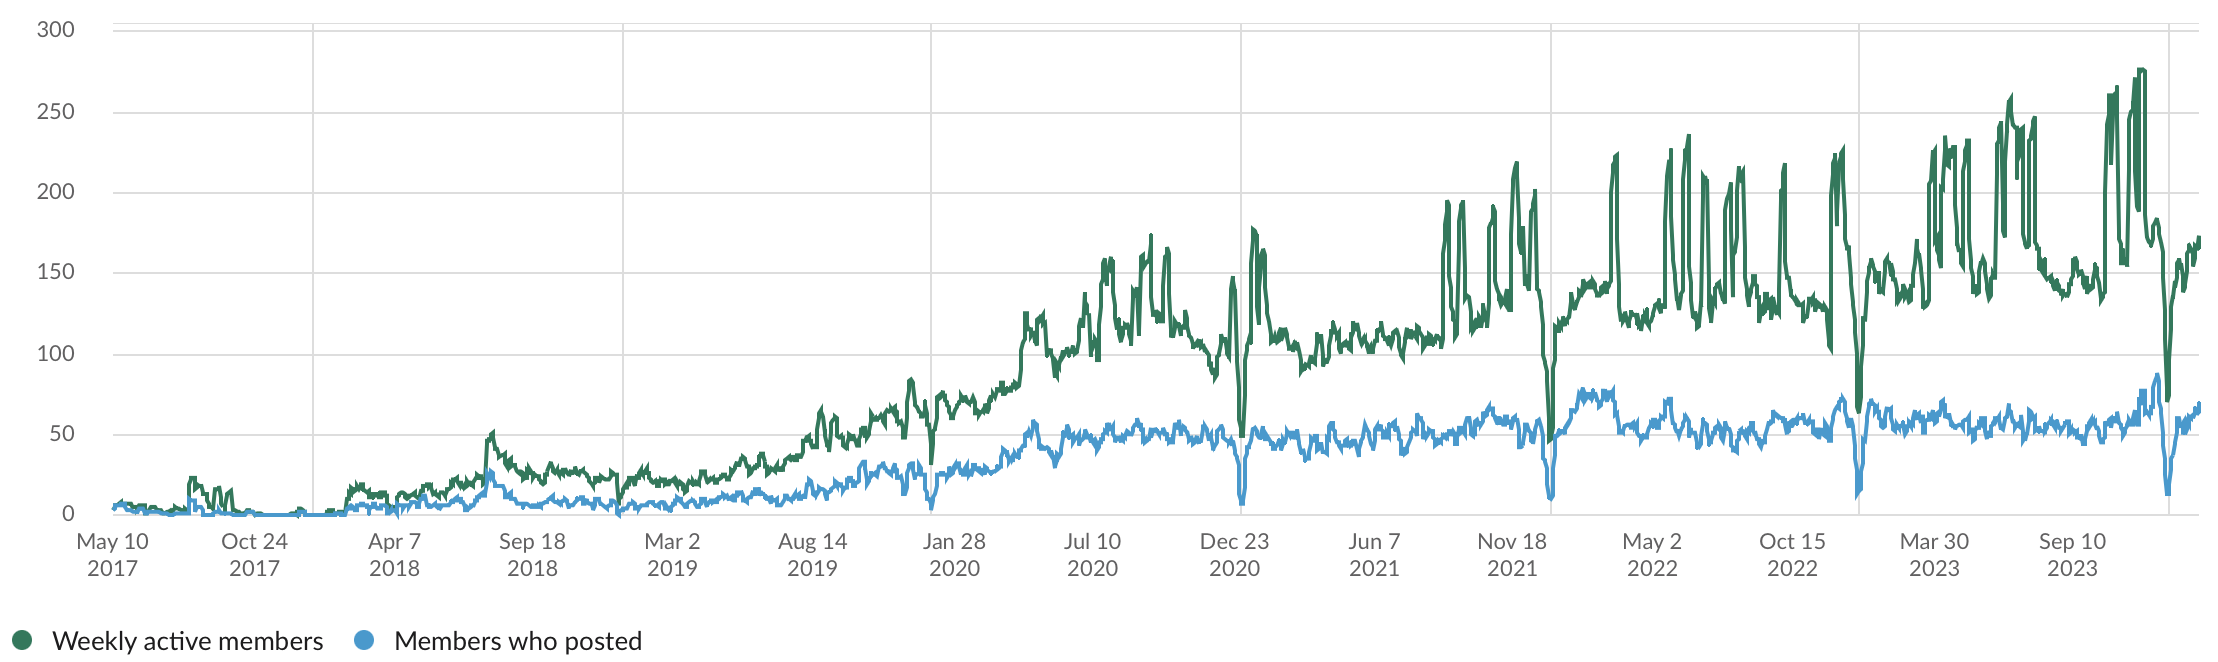
\includegraphics[width=6cm]{figures/KokkosSlack-Users-Feb24}
};
\end{tikzpicture}


\end{frame}


\begin{frame}{The Kokkos Lectures}
        
	\begin{block}{The Kokkos Lectures}
		Join The Kokkos Lectures for a full introduction. 16 hours of lectures with associated exercises as homework.
	\end{block}

\begin{itemize}
	\item \textit{07/17 Module 1: Introduction, Building and Parallel Dispatch}
	\item \textit{07/24 Module 2: Views and Spaces}
	\item 07/31 Module 3: Data Structures + MultiDimensional Loops
	\item 08/07 Module 4: Hierarchical Parallelism
	\item 08/14 Module 5: Tasking, Streams and SIMD
	\item 08/21 Module 6: Internode: MPI and PGAS
	\item 08/28 Module 7: Tools: Profiling, Tuning and Debugging
	\item 09/04 Module 8: Kernels: Sparse and Dense Linear Algebra
        \item 09/11 Reserve Day
\end{itemize}
\end{frame}

\begin{frame}{Find More}

\textbf{Online Resources}:

\begin{itemize}
        \item \url{https://github.com/kokkos}:
                \begin{itemize}
                        \item Primary Kokkos GitHub Organization
                \end{itemize}
        \item \url{https://github.com/kokkos/kokkos-tutorials/wiki/Kokkos-Lecture-Series}:
                \begin{itemize}
			\item{Slides, recording and Q\&A for the Full Lectures}
                \end{itemize}
        \item \url{https://github.com/kokkos/kokkos/wiki}:
                \begin{itemize}
                        \item Wiki including API reference
                \end{itemize}
        \item \url{https://kokkosteam.slack.com}:
                \begin{itemize}
                        \item Slack channel for Kokkos.
                        \item Please join: fastest way to get your questions answered.
                        \item Can whitelist domains, or invite individual people.
                \end{itemize}
\end{itemize}

\end{frame}

\end{document}

